\documentclass[../main.tex]{subfiles}
\begin{document}
\section{K-Nearest Neighbor Model}
In the previous section we analyzed a quite rigid model, now we will move to the K-Nearest Neighbor (k-nn) model, a very flexible approach.\\

The k-nearest neighbors algorithm (k-NN) is a non-parametric method used for classification and regression. In both cases, the input consists of the k closest training examples in the feature space. The output depends on whether k-NN is used for classification or regression. More in details:

K-nn is a \textbf{Lazy} learning algorithm, it store the training data and wait until a test data point is presented, then construct an ad hoc hypothesis to classify that one data point.
\begin{itemize}
    \item It makes \textbf{local estimations} (by locally constant functions) and has not global hypothesis for all the instances, no model to be fit
    \item we need to memorize the input examples
\end{itemize} 
This method is in also called \textbf{distance-based methods}, memory based or instance-based.\\ 




Let take once again the example used for classification, we have seen that applying the linear model seems to make many errors on the training data. let's see what happens when applying a more flexible method like the \textbf{K-nn}.

\begin{figure}[H]
  \centering
  \subfloat[Raw data]{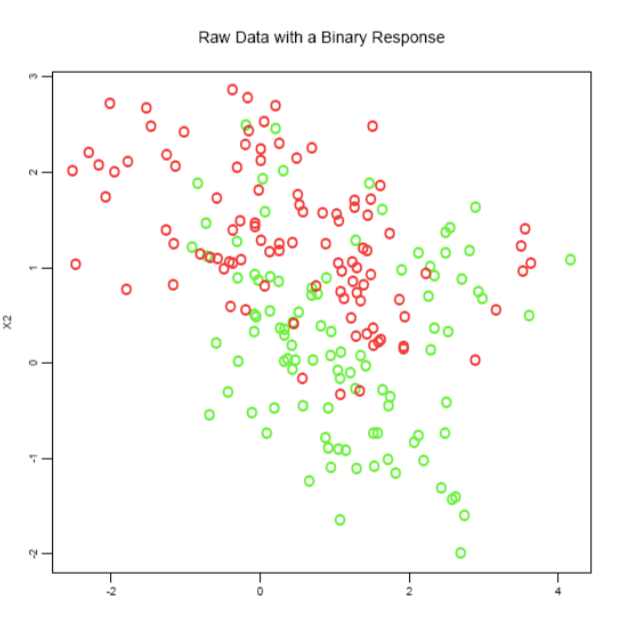
\includegraphics[width=0.45\textwidth]{lectures/2_linear_model/2_classification_example_problem.png}\label{fig:3_classification_example_problem_2}}
  \hfill
  \subfloat[After LMS algorithm]{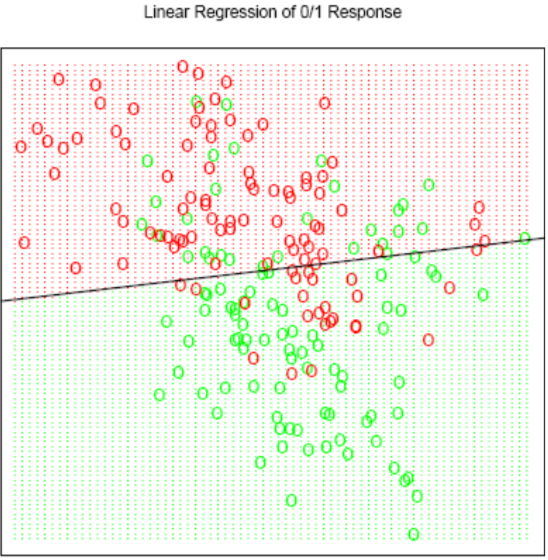
\includegraphics[width=0.45\textwidth]{lectures/2_linear_model/2_classification_example_problem_with_lm.png}\label{fig:3_classification_example_problem_lm_2}}
  \caption{Solution of a classification example with LMS}
\end{figure}

\noindent Let's start to analyze the 1-kk case.\\

\subsection{1-Nearest Neighbor Algorithm}
The algorithm for the 1-nn case is:
\begin{enumerate}
    \item Simply store the training data $<\mathbf{x}_j , y_j>\, ,\; j = 1, \dots, l$
    \item given an input $\mathbf{x}$ (with dimension $n$)
    \item now we want to find the nearest training example $\mathbf{x}_i$:\\
            find the index $i$ s.t. we have the min $d(\mathbf{x},\mathbf{x_i}) \rightarrow i(\mathbf{x}) = \mbox{arg}\min_{j} d(\mathbf{x},\mathbf{x_j})$\\
            
            e.g.  Euclidian distance: $d(\mathbf{x},\mathbf{x_j}) = \sqrt{\sum_{t = 1}^n (x_t - x_{jt})^2} = \norm{\mathbf{x} - \mathbf{x}_j} $ (pattern $\mathbf{x_j}$, component $t$) 
    \item then output $y_i$
\end{enumerate}

\noindent By applying the algorithm to the problem above we can see how this new model works.
The result of the 1-nn algorithm is shown in fig. \ref{fig:3_1nn_eg}\\

\begin{figure}
    \centering
    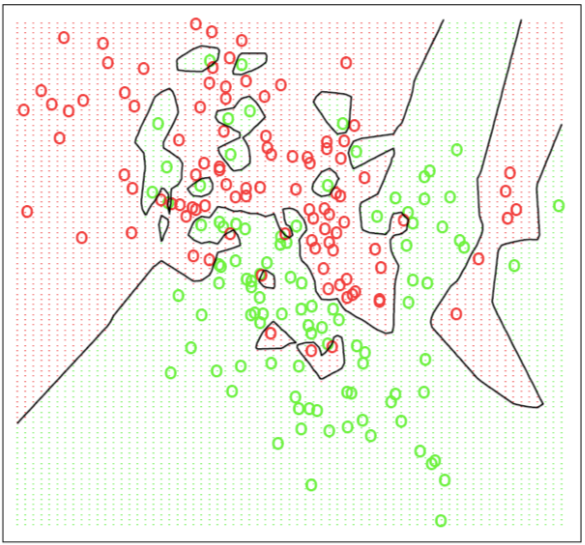
\includegraphics[scale = 0.3]{lectures/3_K_nn/3_1nn_eg.png}
    \caption{1-Nearest Neighbor Classifier}
    \label{fig:3_1nn_eg}
\end{figure}

We can immediately notice that:
\begin{itemize}
    \item the model is very flexible
    \item there is No misclassifications in TR data: $0$ training error. What about the test data?
    \item Decision boundaries is \textbf{not linear}: it is quite \textbf{irregular}
    \item May be unnecessary noisy 
\end{itemize}

\subsection{K-Nearest Neighbors Algorithm}
The algorithm is the same for the 1-nn, here we will extend it to the k-nn case. The output depends on whether k-NN is used for classification or regression: 
\begin{itemize}
    \item \textbf{Regression Case}: take the average.
    $$ avg_k(\mathbf{x}) = 1/k \sum_{\mathbf{x}_i \in N_k(\mathbf{x})}^{} y_i$$
    where $N_k(\mathbf{x})$ is a neighborhood of $\mathbf{x}$ that contains exactly $k$ neighbors (closest patterns according to $d$): k-nearest neighborhood: \textbf{K-nn}.
    
    \item \textbf{Classification Case}: If there is a clear dominance of one of the classes in the neighborhood of an observation $\mathbf{x}$, then it is likely that the observation itself would belong to that class, too. Thus the classification rule is the \textbf{majority voting} among the members of $N_k(\mathbf{x})$:
    \[
    h(\textbf{x}) = \left\{
                \begin{array}{ll}
                  1 \quad if \;\; avg_k(\mathbf{x})>0.5\\
                  0 \quad otherwise
                \end{array}
              \right. \;\;\text{for targets } y \text{ in } \{0,1\} 
    \]
\end{itemize}
So, a natural way to classify a new point is to have a look at its neighbors. Let's see two example:\\

\noindent$\blacksquare$ \textbf{1-nn vs 5-nn example}\\
with two different value of $k$ we can have different classifications (fig. \ref{fig:3_1-nn_vs_5-nn}:
\begin{itemize}
    \item 1-nn return $+$ for $\mathbf{x}_q$
    \item 5-nn return $-$ for $\mathbf{x}_q$
\end{itemize}
Smoothing over a set of neighbors for noisy data.
\begin{figure}[H]
    \centering
    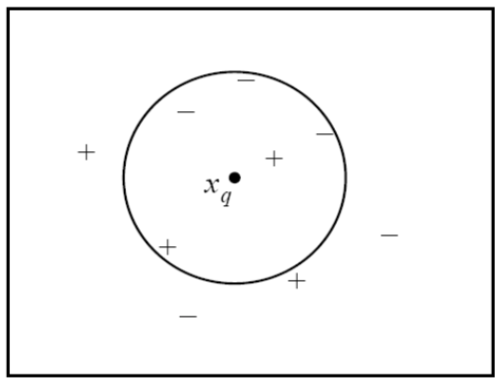
\includegraphics[scale = 0.3]{lectures/3_K_nn/3_1-nn_vs_5-nn.png}
    \caption{1-nn vs 5-nn example}
    \label{fig:3_1-nn_vs_5-nn}
\end{figure}

\noindent$\blacksquare$ \textbf{15-nn example}\\
We can see the result of 15-nn algorithm. Where the predicted class is hence chosen by
majority vote amongst the 15-nearest neighbors.\\

\begin{itemize}
    \item Still very flexible
    \item Some misclassifications in training data
    \item Decision boundaries is not linear: it is still quite, although less, irregular
    \item Decision boundary adapts to the local densities of the classes
\end{itemize}

\begin{figure}
    \centering
    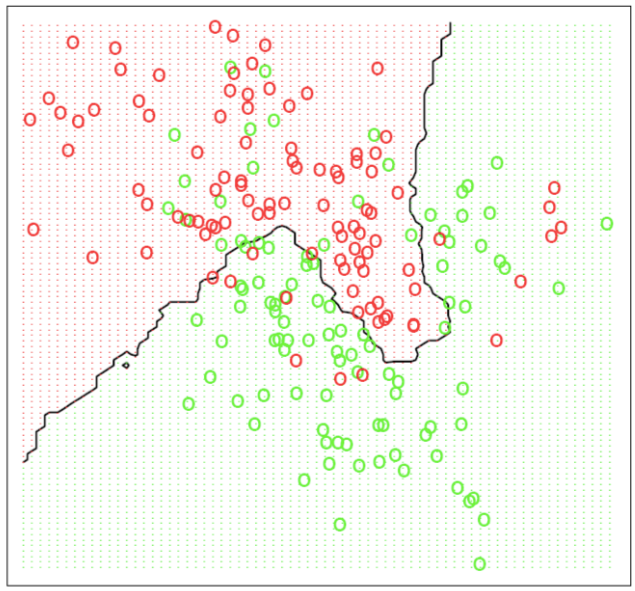
\includegraphics[scale = 0.25]{lectures/3_K_nn/3_15nn_eg.png}
    \caption{15-Nearest Neighbor Classifier}
    \label{fig:3_15nn_eg}
\end{figure}

\noindent$\blacksquare$ \textbf{Voronoi diagram}\\
The Voronoi diagram is implicitly used by K-NN. Each cell consisting of all points closer to $\mathbf{x}$ than to any other patterns. The segments of the Voronoi diagram are all the points in the plane that are equidistant to two patterns. See fig. \ref{fig:voronoi_diagram}
\begin{figure}[h]
    \centering
    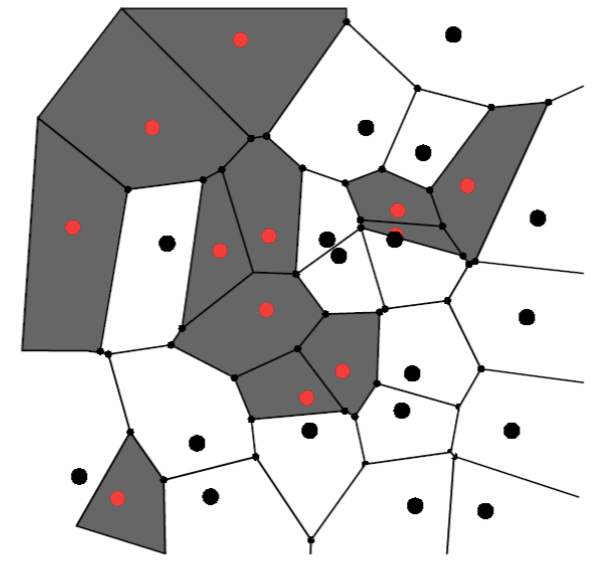
\includegraphics[scale = 0.3]{lectures/3_K_nn/3_voronoi_diagram.png}
    \caption{Voronoi diagram}
    \label{fig:voronoi_diagram}
\end{figure}
\subsection{K-nn for multi-class}
The algorithm is the same used for classification but return the class most common amongst its k nearest neighbors
\[ 
    h(\mathbf{x}) = \mbox{arg}\max_{v} \sum_{\mathbf{x}_i \in N_k(\mathbf{x})}^{}\mathbf{l}_{v, y_i}
\]
\[
    \mathbf{l}_{v, y_i} = \left\{
                \begin{array}{ll}
                  1 \quad if \;\; v = y_i\\
                  0 \quad otherwise
                \end{array}
              \right.
\]

\subsection{K-nn variants: Weighted distance}
It can be useful to weight the contributions of the neighbors, so that the nearer neighbors contribute more to the average than the more distant ones.

\[
    h(\mathbf{x}) = \mbox{arg}\max_{v} \sum_{\mathbf{x}_i \in N_k(\mathbf{x})}^{}\mathbf{l}_{v, y_i} \bullet \frac{1}{d(\mathbf{x},\mathbf{x}_i)^2}
\]

\[
    \mathbf{l}_{v, y_i} = \left\{
                \begin{array}{ll}
                  1 \quad if \;\; v = y_i\\
                  0 \quad otherwise
                \end{array}
              \right.
\]
If $d = 0$ for a $i$, return $y_i$

\subsection{K-nn versus Linear model}
Now we have two different models, they are two extremes of the machine learning panorama, let's to compare them:
\begin{itemize}
    \item The linear model is a rigid model (low variance) and the K-nn is a flexible model (high variance):
    \begin{itemize}
        \item In K-nn with small k, few points can change the decision boundary
        \item We may pay a price for this flexibility
    \end{itemize}
    
    \item Eager versus lazy
    
    \item Parametric versus instance-based
    
    \item global hypothesis for all the instances versus local estimations function (all computation is deferred until classification/regression request) 
\end{itemize}
Given this two scenario:
\begin{itemize}
    \item \textbf{Scenario 1}: The training data in each class were generated from bivariate Gaussian distributions with uncorrelated components and different means.
    \item \textbf{Scenario 2}: The training data in each class came from a mixture of 10 low- variance Gaussian distributions, with individual means themselves distributed as Gaussian.
\end{itemize}

The linear decision boundary from least squares is very smooth, and apparently stable to fit, see fig~\ref{fig:3_classification_example_problem_lm_2}. It does appear to rely heavily on the assumption that a linear decision boundary is appropriate. In language we will develop shortly, it has low variance and potentially high bias.
On the other hand, the k-nearest-neighbor procedures do not appear to rely on any stringent assumptions about the underlying data, and can adapt to any situation, see fig.~\ref{fig:3_1nn_eg} and fig.~\ref{fig:3_15nn_eg}. However, any particular subregion of the decision boundary depends on a handful of input points and their particular positions, and is thus wiggly and unstable—high variance and low bias.\\

Each method has its own situations for which it works best.\\

\noindent$\blacksquare$ \textbf{How many parameters for LM and K-nn}\\

Usually a linear regression model uses $n+1$ parameters (n.b. $\mathbf{x} \in \mathbb{R}^n$) to describe the global function that will fit the training data.\\
It appears that k-nearest-neighbor fits have a single parameter, the number of neighbors $k$, compared to the $n+1$ parameters in least-squares fits. Although this is the case, we will see that the effective number of parameters of k-nearest neighbors is $l/k$ ($l$ is the number of data, in \textit{Hastie} book $l=N$) and is generally bigger than $n+1$, and decreases with increasing $k$.\\

To get an idea of why, note that if the neighborhoods were nonoverlapping, there would be N/k neighborhoods and we would fit one parameter (a mean) in each neighborhood.\\

The error on the training data should be approximately an increasing function of k, and will always be 0 for k = 1.
It is also clear that we cannot use sum-of-squared errors on the training set as a criterion for picking k, since we would always pick k = 1.\\


\noindent$\blacksquare$ \textbf{LS linear vs K-nn with various k values}\\

Figure~\ref{fig:3_degree_of_freedom_plot} shows the results of classifying 10,000 new observations generated from the model and we can observe the misclassification curves for the simulation example used fig~\ref{fig:3_classification_example_problem_lm_2}, fig.~\ref{fig:3_1nn_eg} and fig.~\ref{fig:3_15nn_eg}. We compare the results for least squares and those for k-nearest neighbors for a range of values of k.


Note: how we move from underfitting to overfitting moving the values of K (i.e. the rate $l/k$): more flexibility allows to find the best result if we control “complexity” by K:
\begin{itemize}
    \item \textbf{Underfitting}: $l/k = 1 \;,\; k=l $, in this case the number of nearest-neighbor is equivalent to the number of the data $l$.
    \item \textbf{Overfitting}: $l/k = l \;,\; k=1 $, in this case every sample is nearest-neighbor.
\end{itemize}

\begin{figure}
    \centering
    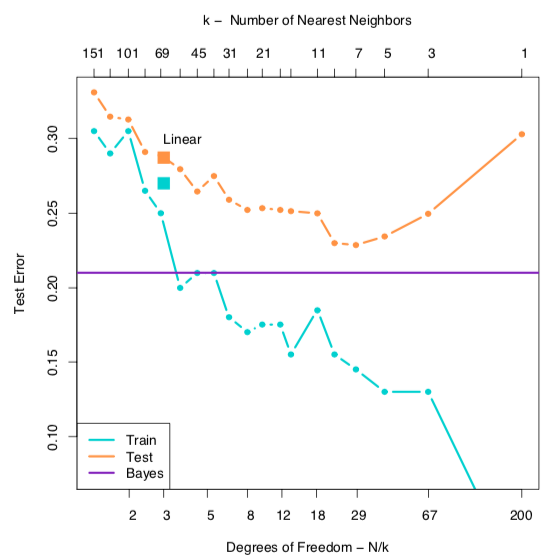
\includegraphics[scale = 0.4]{lectures/3_K_nn/3_degree_of_freedom_plot.png}
    \caption{A single training sample of size 200 was used, and a test sample of size 10,000. The orange curves are test and the blue are training error for k-nearest-neighbor classification. The results for linear regression are the bigger orange and blue squares at three degrees of freedom. The purple line is the optimal Bayes error rate.}
    \label{fig:3_degree_of_freedom_plot}
\end{figure}
\subsection{Bayes Optimal Classifier and K-NN}
Bayes optimal solution (called Bayes classifier):\\

Let's suppose that we know the density $P(x,y)$ we can classifiy to the most probable class, usig the conditional (discrete) distribution as:
\[
    \text{output the class } v \text{ s.t. is max } P(v|\mathbf{x}) \quad (v \; in \; \{C_1, C_2, C_3, \dots, C_k\})
\]

\textbf{ the Bayes rate} is the error rate of the (optimal) Bayes classifier: the minimum achievable error rate given the distribution of the data ( assuming that the generating density is known)

\begin{figure}[H]
  \centering
  \subfloat[Bayes Optimal Classifier]{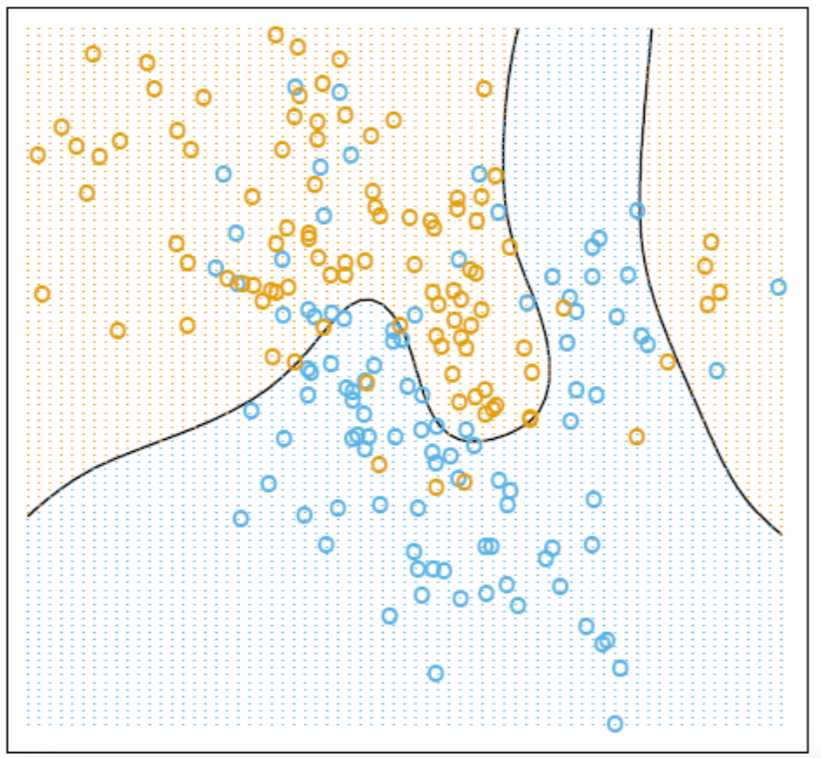
\includegraphics[width=0.45\textwidth]{lectures/3_K_nn/3_bayes_optimal_classifier.png}\label{fig:3_bayes_optimal_classifier}}
  \hfill
  \subfloat[15-nearest neighbors]{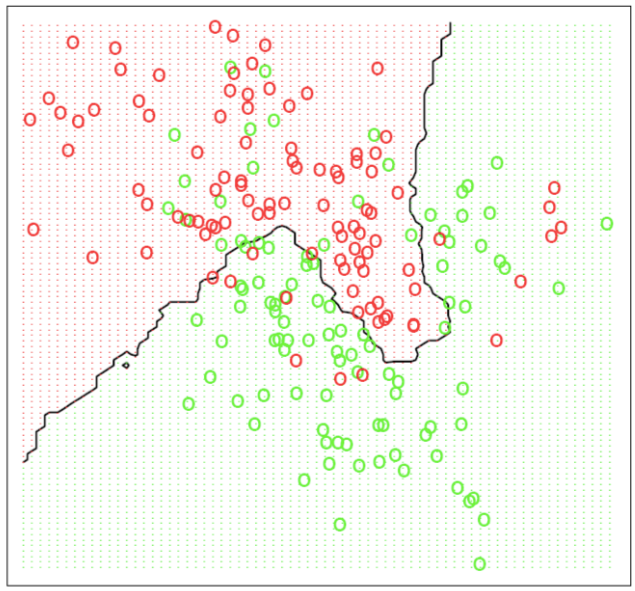
\includegraphics[width=0.45\textwidth]{lectures/3_K_nn/3_15nn_eg.png}\label{fig:3_classification_example_problem_lm_21}}
  \caption{the k-nn classifier directly approximates the solution of a bayes optimal classifier}
\end{figure}

In figure~\ref{fig:3_bayes_optimal_classifier} we can see the optimal Bayes decision boundary for the simulation example. Since the generating density is known for each class, this boundary can be calculated exactly.\\


\textbf{Note on K-NN}: we see that the k-nn classifier directly approximates this solution (a majority vote in a nearest neighborhood amounts to exactly this), except that conditional probability at a point is relaxed to conditional probability within a neighborhood of a point, and probabilities are estimated by training-sample proportions.

\subsection{Inductive Bias of k-nn}
\begin{itemize}
    \item The assumed distance tell us which is the most similar examples
    \item The classification is assumed similar to the classification of the neighbors according to the assumed metric
\end{itemize}

\subsection{Criticism and Limitations}
The K-nn models offer little interpretation:
\begin{itemize}
    \item Subjectivity of interpretation
    \item Dependence on the metric
\end{itemize}
This model has some criticism and limitations, let's see some of them.
\subsubsection{Scale changes and other metrics}
\begin{itemize}
    \item Variable scaling can have an high impact (i.e. k-nn is fragile even with respect to basic preprocessing)
    \begin{figure}[H]
        \centering
        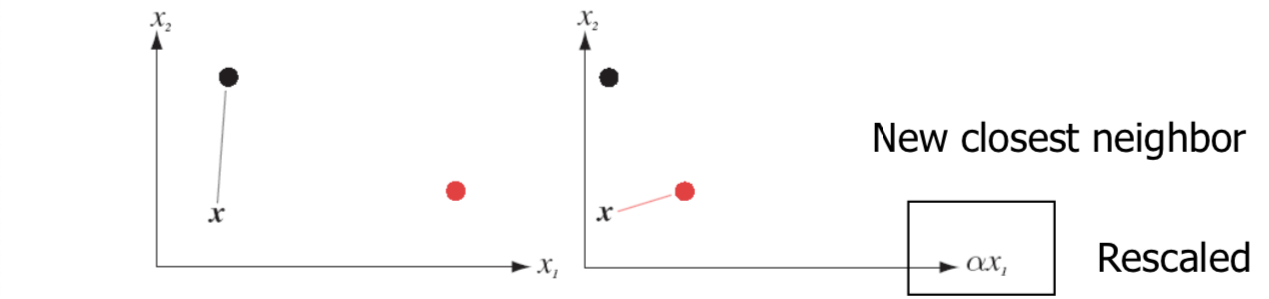
\includegraphics[scale = 0.2]{lectures/3_K_nn/3_scale_and_metrics.png}
    \end{figure}
    Domain knowledge dependent choice. If they should contribute equally: 
    \begin{itemize}
        \item Pay attention to disparity in the ranges of each variables
        \item rescale data to equalize inputs ranges ($\rightarrow$ change the metric)! (E.g. mean zero and variance 1 normalization)
    \end{itemize}
    
    \item Symbolic data require “ad-hoc” metrics (e.g. Hamming distance between two strings of equal length is the number of positions for which the corresponding symbols are different)
\end{itemize}

\subsubsection{Computational cost}
Note that K-nn makes the local approximation to the target function for each new example to be predicted: The computational cost is deferred to the prediction phase!\\

\textbf{Moreover: high retrieval cost}:
computationally intensive for each new input: computing the distances from the test sample to all stored vectors, so the cost in time is proportional to the number of stored patterns and of course there is an high cost in term of space.\\

\textbf{Some Optimization}:
\begin{itemize}
    \item “ad-hoc” proximity search algorithms to optimize
    \item E.g. by indexing the patterns
\end{itemize}

\subsubsection{Curse of Dimensionality}
We have examined two learning techniques for prediction so far: the stable but biased linear model and the less stable but apparently less biased class of k-nearest-neighbor estimates. It would seem that with a reasonably large set of training data, we could always approximate the theoretically optimal conditional expectation by k-nearest-neighbor averaging, since we should be able to find a fairly large neighborhood of observations close to any x and average them. This approach and our intuition breaks down in high dimensions, and the phenomenon is commonly referred to as the \textbf{curse of dimensionality} (Bellman, 1961). There are many manifestations of this problem, and we will examine a few here.

\begin{enumerate}
    \item \textbf{It is hard to find nearby points in high dimensions}:\\
    K-nearest neighbors can fail in high dimensions, because it becomes difficult to gather K observations close to a target (query) point $\mathbf{x}_q$: 
    \begin{itemize}
        \item near neighborhoods tend to be spatially large, and estimates are not longer local
        \item Reducing the spatial size of the neighborhood means reducing K, and the variance of the estimate increases ($\rightarrow$ overfitting).
    \end{itemize}
    
    \begin{figure}
        \centering
        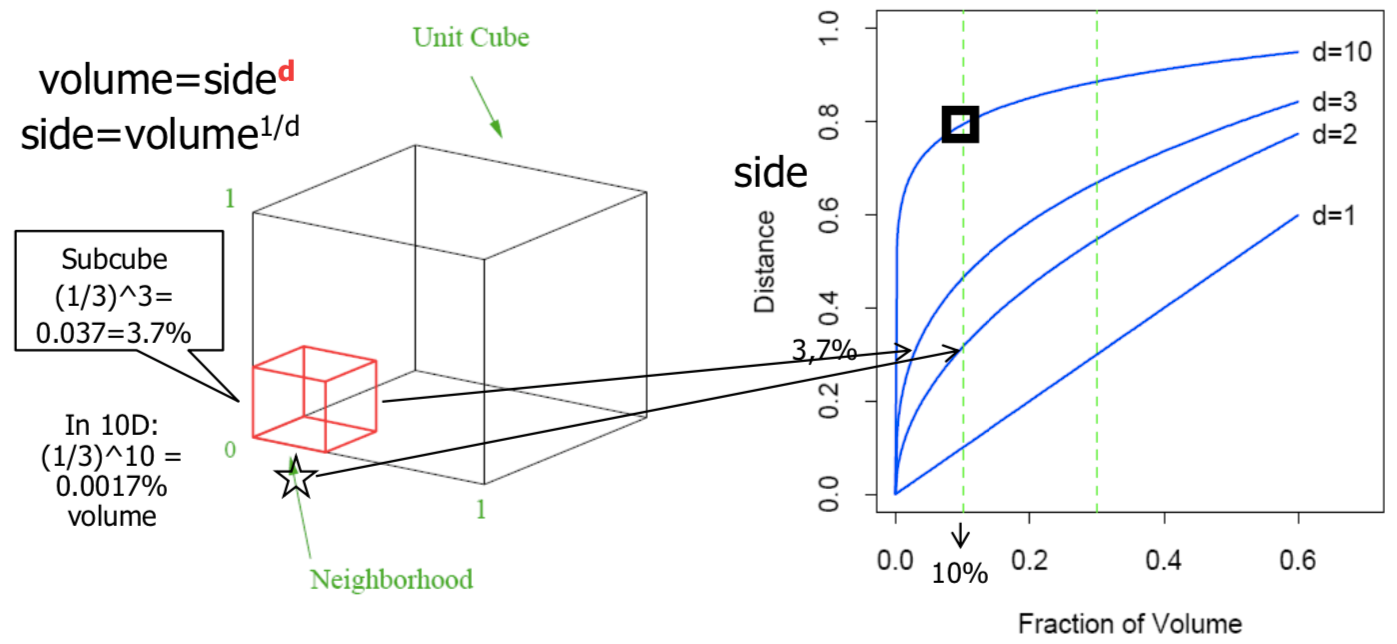
\includegraphics[scale = 0.2]{lectures/3_K_nn/3_curse_of_dim_hypercube.png}
        \caption{The curse of dimensionality is well illustrated by a subcubical neighborhood for uniform data in a unit cube. The figure on the right shows the side-length ( $r^{1/d}$) of the subcube needed to capture a fraction r of the volume of the data, for different dimensions d. In ten dimensions we need to cover 80\% of the range of each coordinate to capture 10\% of the data. (since $0.1^{1/10}=~ 0.8$), while in 2D 30\% (0.316 sidelenght) was sufficient.}
        \label{fig:3_curse_of_dim_hypercube}
    \end{figure}
    Consider the nearest-neighbor procedure for inputs uniformly distributed in a p-dimensional unit hypercube, as in Figure~\ref{fig:3_curse_of_dim_hypercube}. Suppose we send out a hypercubical neighborhood about a target point to capture a fraction r of the observations. Since this corresponds to a fraction r of the unit volume, the expected edge length will be $ep(r) = r^{1/d}$. In ten dimensions $e_{10}(0.01) = 0.63$ and $e_{10}(0.1) = 0.80$, while the entire range for each input is only 1.0. So to capture 1\% or 10\% of the data to form a local average, we must cover 63\% or 80\% of the range of each input variable. Such neighborhoods are no longer “local.” Reducing r dramatically does not help much either, since the fewer observations we average, the higher is the variance of our fit.\\
    
    \textbf{Further explanation}:
    Image that to have K data you need 10\% of the volume. How much sidelength do you need? From 30\% to 80\% moving from 2D to 10D.\\
    
    On the other side:
    \begin{itemize}
        \item 1D: with 0.3 sidelength we take 30\% of data volume
        \item 2D: with 0.3 sidelength we take 10\% of data volume (the red square)
        \item 3D: with 0.3 sidelength we take 3.7\% of data volume (the red cube)
        \item 10D: with 0.3 sidelength we take 0.0017\% of data volume.
    \end{itemize}
    This sidelength is not sufficient to have K data, unless we use small K (which can lead to overfitting)
    
    \item \textbf{Low sampling density for high-dim data}\\
    Sampling density is proportional to $l^{1/d}$ ($l$ data, $d=dim$).
    
    Another manifestation of the curse is that the sampling density is proportional to  $l^{1/d}$, where $d$ is the dimension of the input space and $l$ is the number of samples. Thus, if $l = 100$ represents a dense sample for a single input problem and 100 points are sufficient to estimate a function in $\mathbb{R}^1$, then $l = 100^{10}$ is the sample size required for the same sampling density with 10 inputs (to achieve similar accuracy in $\mathbb{R}^{10}$ (10-dim input). Thus in high dimensions all feasible training samples sparsely populate the input space.
    
    \item \textbf{Irrelevant features: The Curse of Noisy}
    if the target depends on only few of many features in x (e.g. 2 out 20), we could retrieve a “similar pattern” with the similarity dominated by the large number of irrelevant features. It grows with the dimensionality.
    
    
    \item \textbf{All sample points are close to an edge of the sample (From \textit{Hastie}}
    Another consequence of the sparse sampling in high dimensions is that all sample points are close to an edge of the sample. Consider N data points uniformly distributed in a d-dimensional unit ball centered at the origin. Suppose we consider a nearest-neighbor estimate at the origin. The median distance from the origin to the closest data point is given by the expression:
    $$ d(d,l) = \left(1 - \frac{1^{1/l}}{2}\right)^{1/d}$$
    A more complicated expression exists for the mean distance to the closest point. For $l = 500$, $d = 10$ , $d(d,l) \approx	0.52$, more than halfway to the boundary. Hence most data points are closer to the boundary of the sample space than to any other data point. The reason that this presents a problem is that prediction is much more difficult near the edges of the training sample. One must extrapolate from neighboring sample points rather than interpolate between them.
\end{enumerate}

\subsection{An improvement}
Irrelevant features:\\
We may weights features according to their relevance
\begin{itemize}
    \item Stretching the axes along some dimension
    \item Weights can be searched by a (expensive) model selection approach or other approaches ...
\end{itemize}
Feature selection approaches: eliminates some variables $\rightarrow$ reduce input dimension

\subsection{other local models in ML}
\begin{itemize}
    \item Kernel smoothers
    \item Local linear regression
    \item Prototype methods
    \item Case-basedreasoning
\end{itemize}

\subsection{Summary: K-nn design choices}
\begin{itemize}
    \item The distance metric to measure the closeness between patterns (e.g. Euclidian, Hamming, Manhattan distance..., weights on input features). Often this is the key for a successful applications!
    \item K (number of neighbors: control underfitting/overfitting)
\end{itemize}

Often necessary to select:
\begin{itemize}
    \item A subset of data (set of prototypes): e.g by clustering
    \item A subset of features
\end{itemize}
Various approaches to deal with the issues mentioned above.
\newpage
\begin{figure}[H]
    \centering
    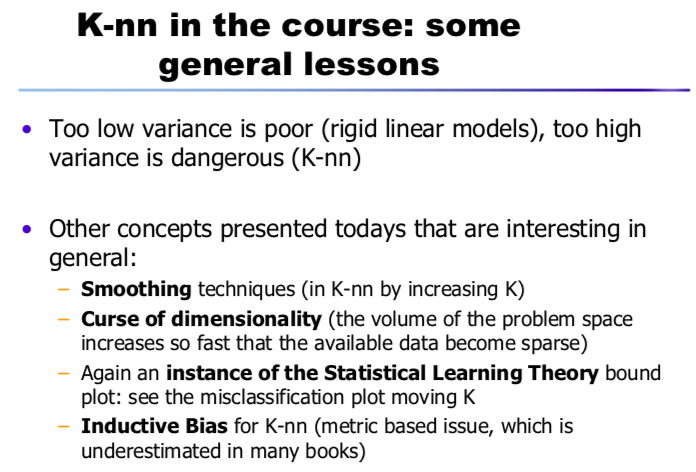
\includegraphics[scale = 0.5]{lectures/3_K_nn/3_knn_end1.png}
\end{figure}

\begin{figure}[H]
    \centering
    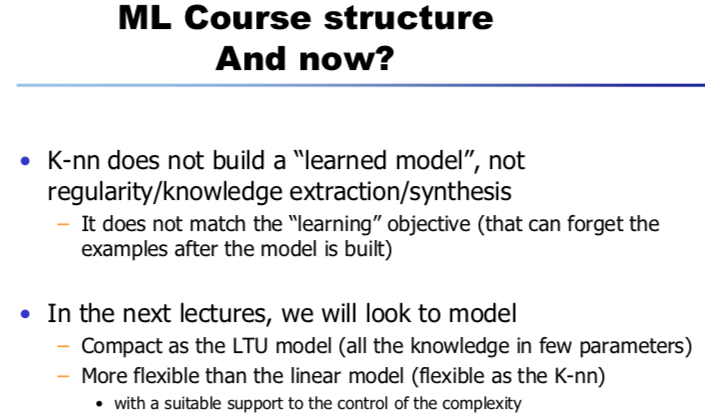
\includegraphics[scale = 0.5]{lectures/3_K_nn/3_knn_end2.png}
\end{figure}
\end{document}
